\section{Results}
\label{sec:results}

This section covers what significance of the approach to collecting
runtime application I/O data and how the new analyses helped provide
more insight into I/O behavior. Figure \ref{a}

\RED{ADD 1 or 2 plots of HACC application for opens and closes as well (interesting results in Grafana)}


Figure \ref{f:mpi_io} shows the duration of the reads and writes per
rank for each execution (\texttt{job\_id} metric) of the MPI-IO
benchmark without using collective operations. We notice a similar
behavior for the I/O operations duration for all jobs except the
second one. It presents a mean duration of 6.75 seconds for reads and
78s for writes, while the other jobs had a mean duration of 0.05s for
reads and 54s for writes. In fact, a single application can have
multiple unique I/O behavior that can degradate the performance of the
application \cite{costa2021}. With the collected logs, we can perform
a spatial performance analysis to understand the variability in the
I/O behavior per system component, in this case, per nodes and
ranks. 

\begin{figure}
	\centering
	% 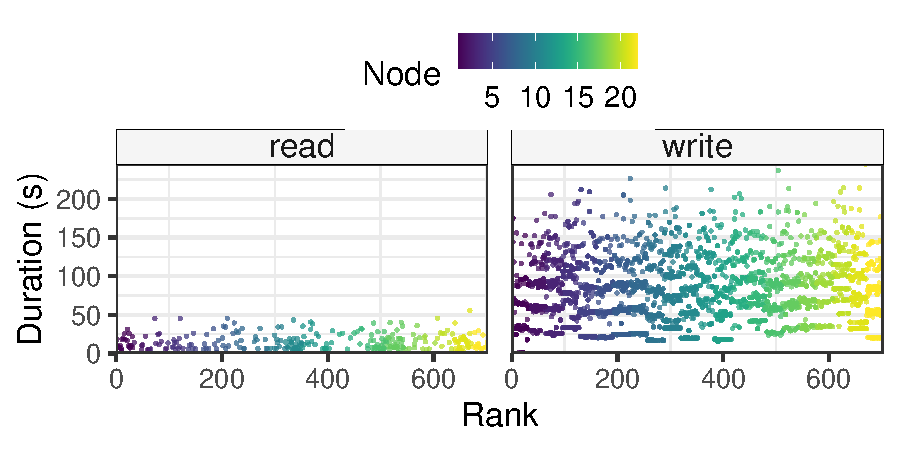
\includegraphics[width=\linewidth]{figs/255653_mpi_io_luster_no_coll_duration.pdf}
        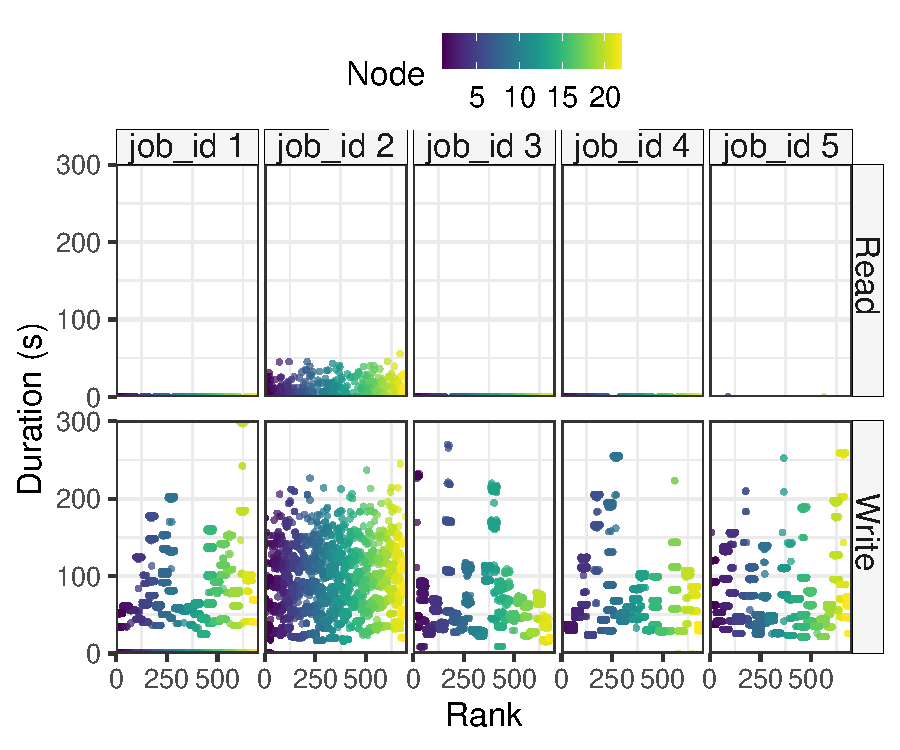
\includegraphics[width=\linewidth]{figs/mpi_io_luster_no_coll_duration_allexperiments.pdf}
	\caption{Jobs for the MPI-IO benchmark without collective
          operations presented variability in the number and duration
          of I/O operations.}
	\label{f:mpi_io}
      \end{figure}

      We can temporaly view the occurences of writes and read
      throughout the total application execution time, and correlate
      with other log informations, such as the ranks perform I/O
      operations and their durations.

\begin{figure}
	\centering
	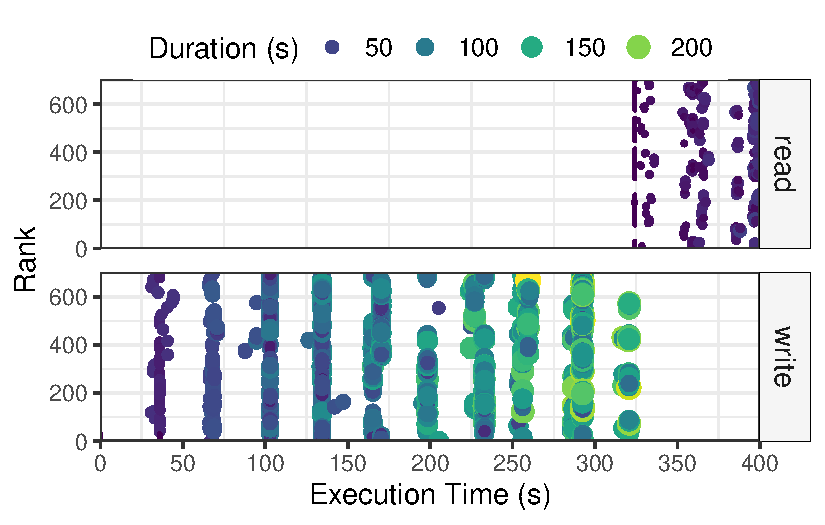
\includegraphics[width=\linewidth]{figs/255653_mpi_io_luster_no_coll_execution2.pdf}
	\caption{Distribution of reads and writes operations
          throughout the execution time, with respective
          durations. The application performs writings during ten
          phases, and then reads at the end.}
	\label{f:mpi_io}
\end{figure}

\begin{figure*}
	\centering
	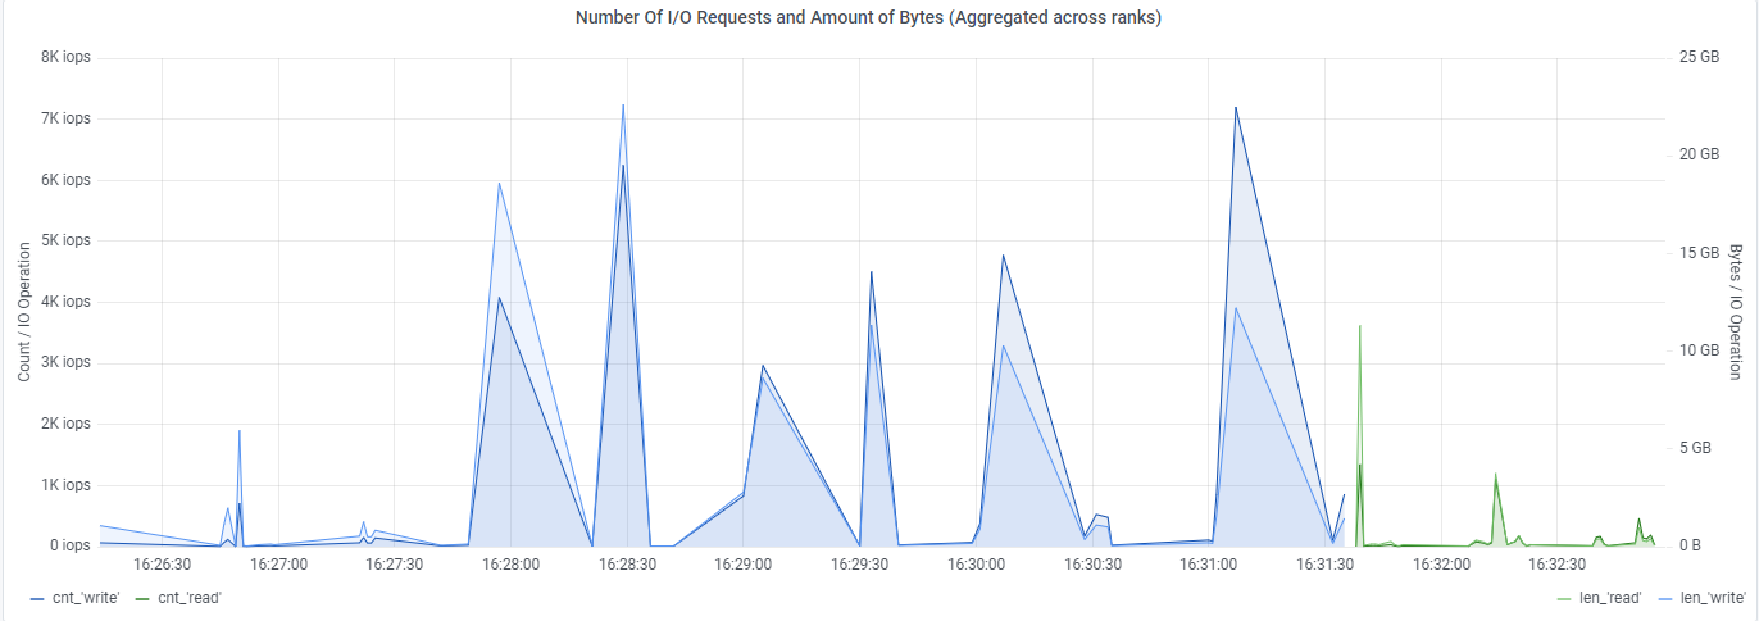
\includegraphics[width=\textwidth]{figs/255653_mpi_io_luster_no_coll.pdf}
	\caption{MPI-IO without collective operations. Graphana visualization using temporal data collected
          with Darshan LDMS}
	\label{f:CSV Header and Output}
      \end{figure*}

 \RED{ADD text about the 3 plots building a narrative how the
   timestamps show valuable insights and we can also see this behavior
 on Grafana.}